\documentclass[
  bibliography=totoc,     % Literatur im Inhaltsverzeichnis
  captions=tableheading,  % Tabellenüberschriften
  titlepage=firstiscover, % Titelseite ist Deckblatt
]{scrartcl}

% Paket float verbessern
\usepackage{scrhack}

% Warnung, falls nochmal kompiliert werden muss
\usepackage[aux]{rerunfilecheck}

% deutsche Spracheinstellungen
\usepackage{polyglossia}
\setmainlanguage{german}

% unverzichtbare Mathe-Befehle
\usepackage{amsmath}
% viele Mathe-Symbole
\usepackage{amssymb}
% Erweiterungen für amsmath
\usepackage{mathtools}

% Fonteinstellungen
\usepackage{fontspec}
% Latin Modern Fonts werden automatisch geladen

\usepackage[
  math-style=ISO,    % ┐
  bold-style=ISO,    % │
  sans-style=italic, % │ ISO-Standard folgen
  nabla=upright,     % │
  partial=upright,   % ┘
  warnings-off={           % ┐
    mathtools-colon,       % │ unnötige Warnungen ausschalten
    mathtools-overbracket, % │
  },                       % ┘
]{unicode-math}

% traditionelle Fonts für Mathematik
\setmathfont{Latin Modern Math}
\setmathfont{XITS Math}[range={scr, bfscr}]
\setmathfont{XITS Math}[range={cal, bfcal}, StylisticSet=1]

% Zahlen und Einheiten
\usepackage[
  locale=DE,                 % deutsche Einstellungen
  separate-uncertainty=true, % immer Fehler mit \pm
  per-mode=reciprocal,       % ^-1 für inverse Einheiten
  output-decimal-marker=.,   % . statt , für Dezimalzahlen
]{siunitx}

% chemische Formeln
\usepackage[
  version=4,
  math-greek=default, % ┐ mit unicode-math zusammenarbeiten
  text-greek=default, % ┘
]{mhchem}

% richtige Anführungszeichen
\usepackage[autostyle]{csquotes}

% schöne Brüche im Text
\usepackage{xfrac}

% Standardplatzierung für Floats einstellen
\usepackage{float}
\floatplacement{figure}{htbp}
\floatplacement{table}{htbp}

% Floats innerhalb einer Section halten
\usepackage[
  section, % Floats innerhalb der Section halten
  below,   % unterhalb der Section aber auf der selben Seite ist ok
]{placeins}

% Seite drehen für breite Tabellen
\usepackage{pdflscape}

% Captions schöner machen.
\usepackage[
  labelfont=bf,        % Tabelle x: Abbildung y: ist jetzt fett
  font=small,          % Schrift etwas kleiner als Dokument
  width=0.9\textwidth, % maximale Breite einer Caption schmaler
]{caption}
% subfigure, subtable, subref
\usepackage{subcaption}

% Grafiken können eingebunden werden
\usepackage{graphicx}
% größere Variation von Dateinamen möglich
\usepackage{grffile}

% schöne Tabellen
\usepackage{booktabs}

% Verbesserungen am Schriftbild
\usepackage{microtype}

% Literaturverzeichnis
\usepackage[
  backend=biber,
]{biblatex}
% Quellendatenbank
\addbibresource{lit.bib}
\addbibresource{programme.bib}

% Hyperlinks im Dokument
\usepackage[
  unicode,        % Unicode in PDF-Attributen erlauben
  pdfusetitle,    % Titel, Autoren und Datum als PDF-Attribute
  pdfcreator={},  % ┐ PDF-Attribute säubern
  pdfproducer={}, % ┘
]{hyperref}
% erweiterte Bookmarks im PDF
\usepackage{bookmark}

% Trennung von Wörtern mit Strichen
\usepackage[shortcuts]{extdash}

\author{
  Timo Gräßer
  \texorpdfstring{
    \\
    \href{mailto:timo.graesser@udo.edu}{timo.graesser@udo.edu}
  }{}%
  \texorpdfstring{\and}{, }
  Jasper Karl Lammering%
  \texorpdfstring{
    \\
    \href{mailto:jasper.lammering@udo.edu}{jasper.lammering@udo.edu}
  }{}%
}
\publishers{TU Dortmund – Fakultät Physik}

\ExplSyntaxOn
 \NewDocumentCommand \g {m}
 {
  \ensuremath{
    \symup{#1}
  }
 }
 \ExplSyntaxOff


\subject{V354}
\title{Gedämpfte und erzwungene Schwingungen}
\date{
  Durchführung: 8.12.2015
  \hspace{3em}
  Abgabe: 15.12.2015
}

\begin{document}

\maketitle
\thispagestyle{empty}
\tableofcontents
\newpage

\section{Einleitung}
Im folgenden Versuch werden verschiedene Schwingungszustände in einem RCL-Kreis
untersucht.

\section{Theorie}
\label{sec:Theorie}

\subsection{Gedämpfte Schwingungen}

Ein gedämpfter elektrischer Schwingkreis ist beispielsweise ein \textbf{RCL}-Kreis.
In Abbildung \ref{fig:rcl} ist einer abgebildet.
Dort schwingt die elektrische Energie zwischen dem Kondensator und der Spule
hin und her. Doch am Widerstand wird ein Teil der Energie in Wärmeenergie umgewandelt.
So wird dem System Energie entzogen und die Schwingungsamplitude nimmt ab.

\begin{figure}[h]
  \centering
  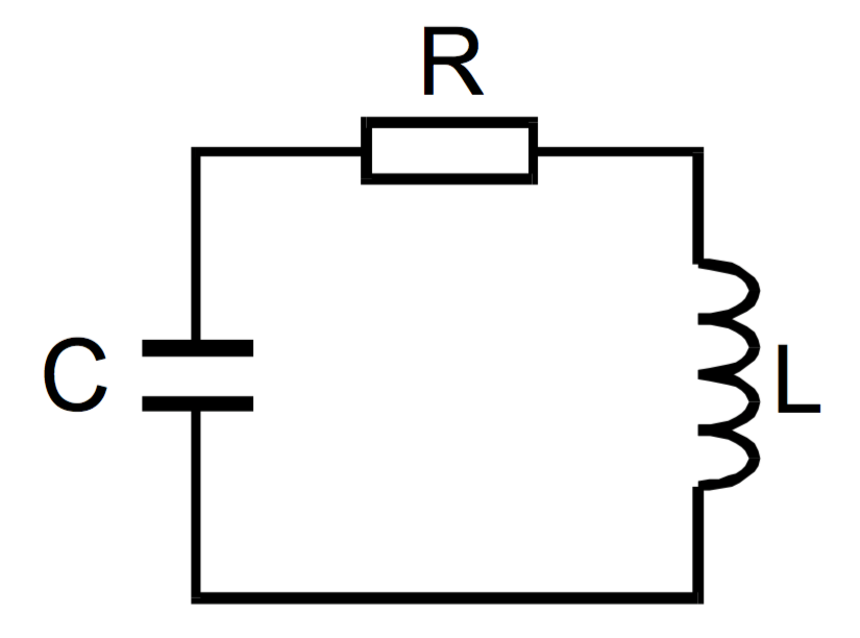
\includegraphics[height = 3 cm]{RCL.pdf}
  \caption{Eine \textbf{RCL}-Schaltung \cite{anleitung}.}
  \label{fig:rcl}
\end{figure}

Über das 2.Kirchhoffsche Gesetz, dass die Summe aller Spannungen null ist, ergibt
sich folgende Differentialgleichung:

\begin{equation}
  \frac{\symup{d}^2 \g{I}}{\symup{d t}^2} + \frac{\symup{R}}{\symup{L}}
  \frac{\g{d I}}{\g{d t}} + \frac{1}{\g{L C}} \g{I} = 0.
  \label{eqn:dgl}
\end{equation}

Als Lösungen ergeben sich die folgenden:

\begin{equation}
  \mathfrak{I}(t) = \mathfrak{U}_1 \textbf{e}^{\g{i\tilde{\omega}_1t}} + \mathfrak{U}_2
  \textbf{e}^{\g{i\tilde{\omega}_2t}}.
\end{equation}

$\mathfrak{U}_1$ und $\mathfrak{U}_2$ sind hierbei beliebige komplexe Zahlen.
$\g{\tilde{\omega}}_\text{1}$ und $\g{\tilde{\omega}}_\text{1}$ sind Konstanten nach Gleichung
\eqref{eqn:konstant}.

\begin{equation}
  \tilde{\omega}_{1,2} = \g{i\frac{R}{2 L} \pm \sqrt{\frac{1}{L C} - \frac{R^2}{4 L^2}}}
  \label{eqn:konstant}
\end{equation}

Mit den Abkürzungen

\begin{align}
  2 \pi \mu := \g{\frac{R}{2 L}} & \text{und} & 2 \pi \g{\tilde{\nu}} := \g{\sqrt{\frac{1}{L C} - \frac{R^2}{4 L^2}}}
\end{align}

ergibt sich die Gleichung \eqref{eqn:gedschw}.

\begin{equation}
  I(t) = A_0 \g{e}^{-2 \g{\pi} \mu t} \cos(2 \g{\pi} \nu t + \eta)
  \label{eqn:gedschw}
\end{equation}

Klar zu erkennen ist hier die Oszillation und die exponentielle Abnahme.
In Abbildung \ref{fig:gedschw} ist dies auch zu erkennen.

\begin{figure}[h]
  \centering
  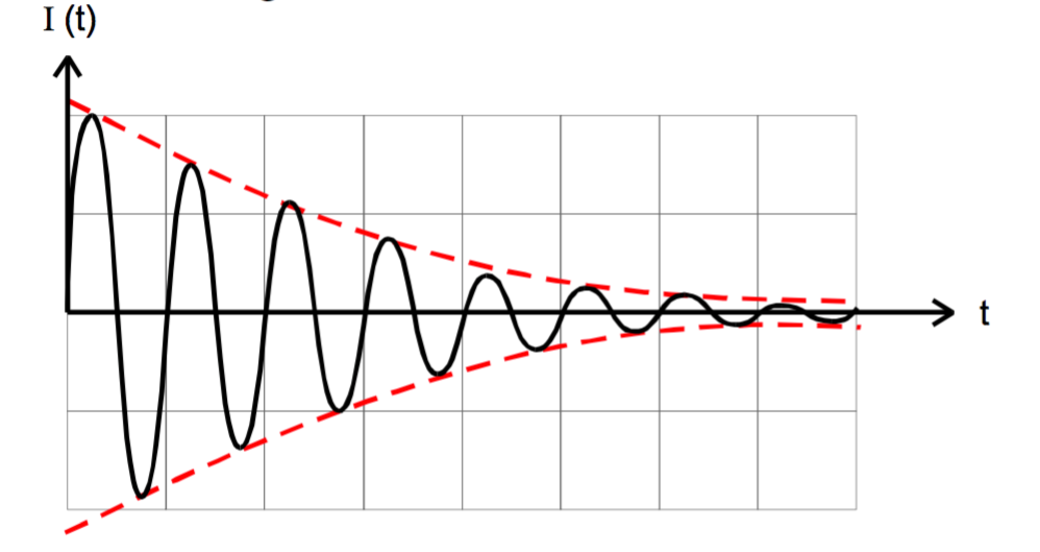
\includegraphics[width = \textwidth]{gedschw.pdf}
  \caption{Eine gedämpfte Schwingung mit der Einhüllenden $\pm e^{-2\g{\pi}\mu t}$.}
  \label{fig:gedschw}
\end{figure}

 \section{Durchführung}
\label{sec:Durchführung}

\subsection{Gedämpfte Schwingungen}
\label{sec:durchgedschw}

Aufgabe ist es in diesem Abschnitt der Messung die Abklingzeit der gedämpften
Schwingung zu bestimmen und dann den effektiven Dämpfungswiderstand $R_{\text{eff}}$
zu berechnen.
Der Versuchsaufbau ist in Abbildung \ref{fig:schalta} zu sehen.

%schaltung a hier
\begin{figure}[h]
  \centering
  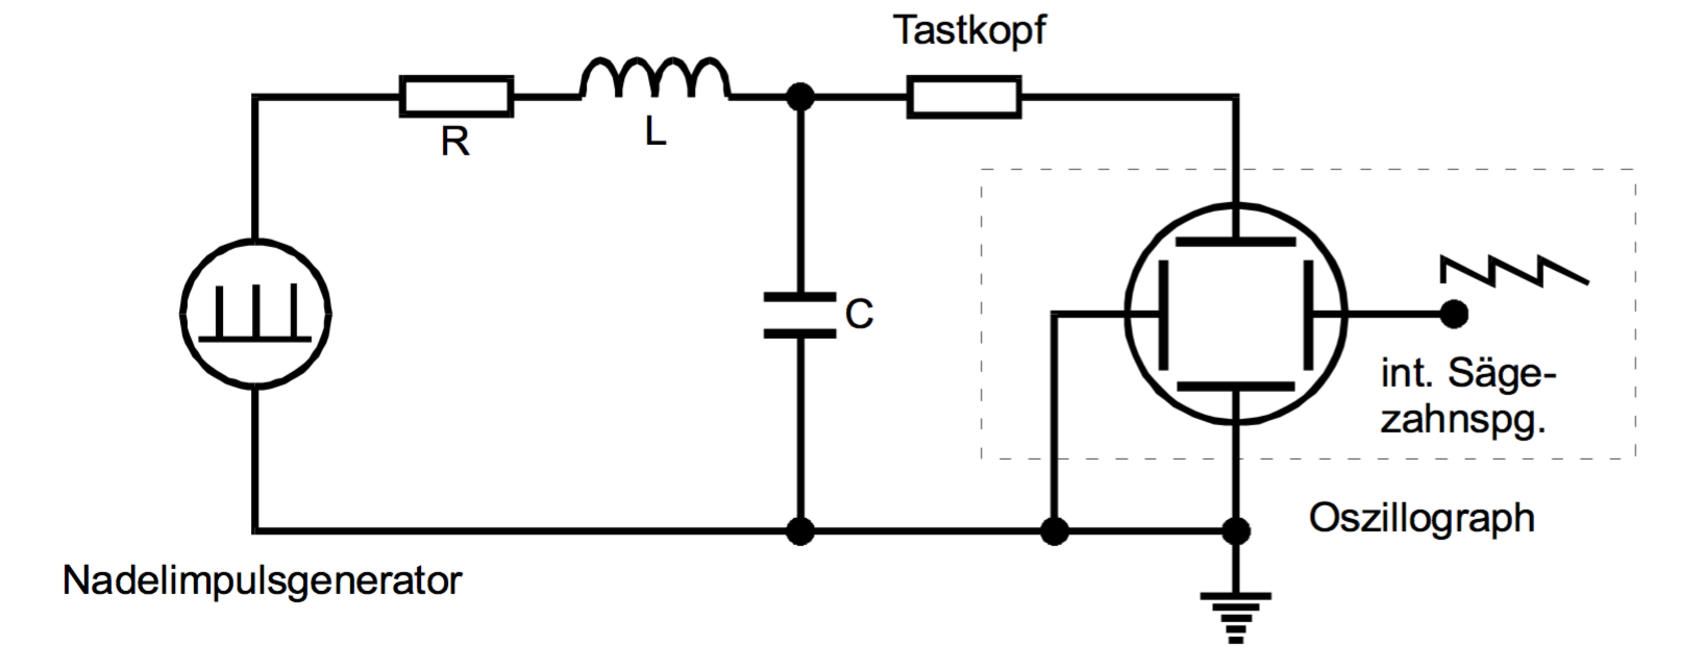
\includegraphics[width = \textwidth]{Schaltunga.pdf}
  \caption{Schaltung zur Bestimmung des effektiven Dämpfungswiderstands \cite{anleitung}.}
  \label{fig:schalta}
\end{figure}

Als Widerstand wird $R~=~\SI{682 +- 1}{\ohm}$ benutzt. Die Spule hat
die Impedanz $L~=~\SI{16.78 +- 0.09}{\milli\henry}$, der Kondensator besitzt
den Wert $C~=~\SI{2.066 +- 0.006}{\nano\farad}$.

Die Spannungsquelle liefert eine Rechteckspannung. Abgegriffen wird diese,
wie dargestellt, mit einem Tastkopf, der einen hohen Innenwiderstand
$R_{\text{i}}~=~\SI{10}{\mega\ohm}$ hat. Dann werden die Werte vom digitalen
Oszilloskop mit einem USB-Stick entnommen.

\subsection{Aperiodischer Grenzfall}

Nun wird der Widerstand $R_{\text{ap}}$ bestimmt, bei dem das Oszilloskop
eine exponentielle Abnahme der Spannung anzeigt.

%schaltung b hier
\begin{figure}[h]
  \centering
  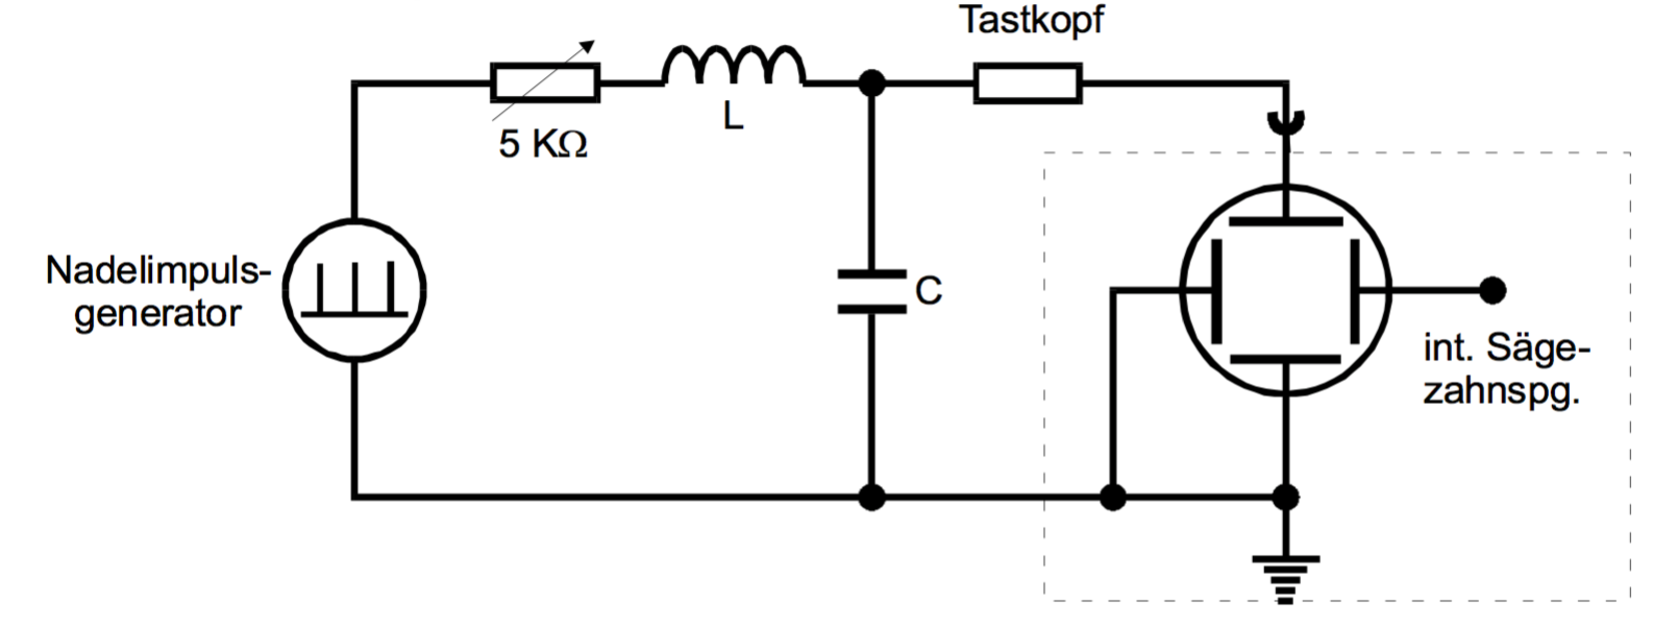
\includegraphics[width = \textwidth]{Schaltungb.pdf}
  \caption{Schaltung zur Bestimmung von $R_{\text{ap}}$ \cite{anleitung}.}
  \label{fig:schaltb}
\end{figure}

In Abbildung \ref{fig:schaltb} ist zu erkennen, dass ein ähnlicher
Versuchsaufbau wie in Kapitel \ref{sec:durchgedschw} benutzt wird.
Die oben erwähnten Bauteile sind die selben und haben auch die selben Werte.
Nur der Widerstand $R$ ist in diesem Falle regelbar bis zu einem Maximum
von $\SI{5}{\kilo\ohm}$.

Um $R_{\text{ap}}$ zu finden wird er auf die maximalen $\SI{5}{\kilo\ohm}$
eingestellt und dann verringert, bis ein Überschwingen der Kurve auf dem
Schirm des Oszillographen zu beobachten ist. Dann wird $R$ wieder etwas
vergrößert, bis die Überschwingung verschwindet. $R_{\text{ap}}$ ist dann
gefunden und wird notiert

\subsection{Erzwungene Schwingungen}

In diesem Teil der Messung werden die Frequenzabhängigkeit der Kondensatorspannung
und der Phase zwischen Erreger- und Kondensatorspannung untersucht.

Dazu wird die Schaltung aus Abbildung \ref{fig:schaltcd} benutzt.

%schaltung cd hier
\begin{figure}[h]
  \centering
  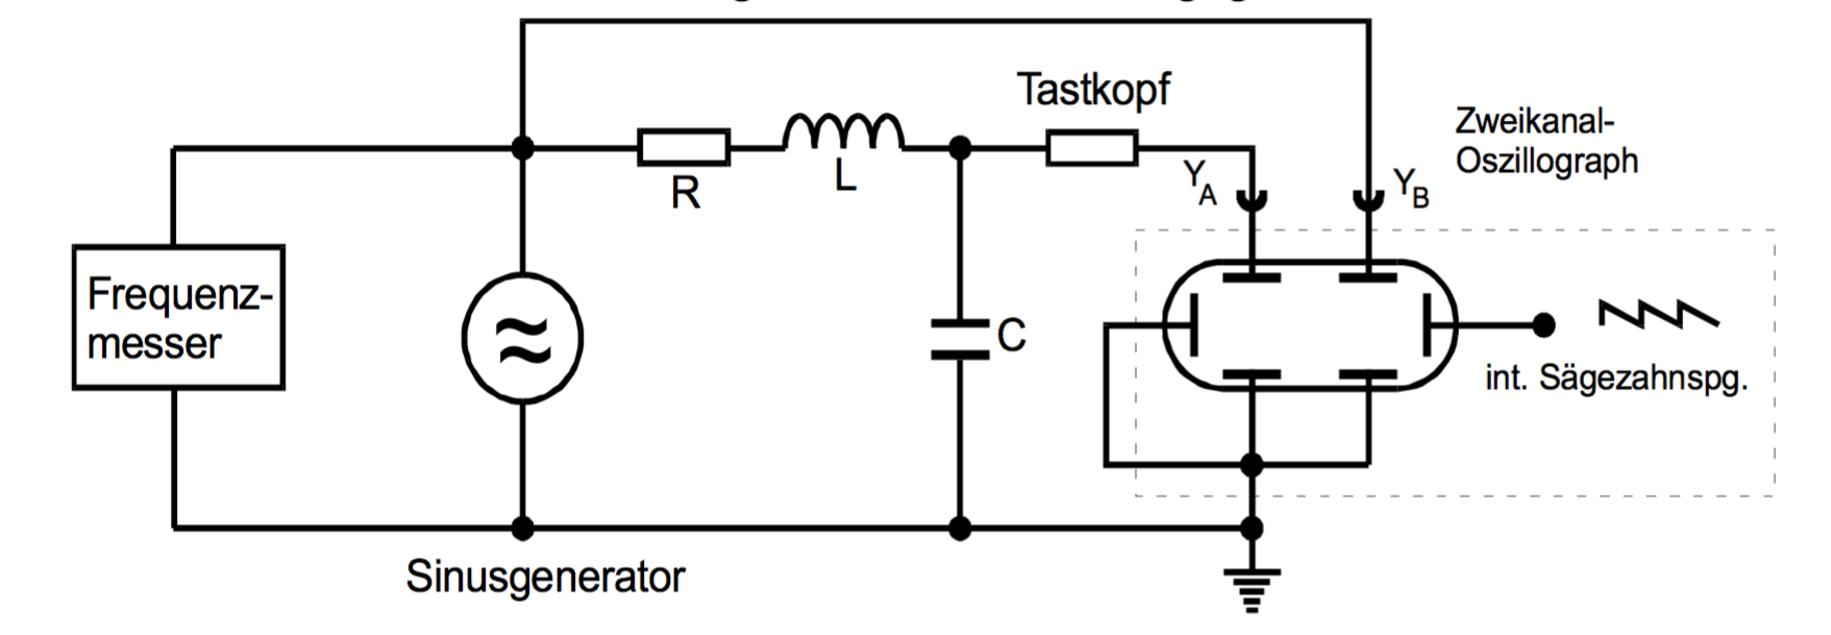
\includegraphics[width = \textwidth]{Schaltungcd.pdf}
  \caption{Schaltung zur Bestimmung von $U_C(\omega)$ und $\varphi(\omega)$ \cite{anleitung}.}
  \label{fig:schaltcd}
\end{figure}

Die Werte für $C$ und $L$ sind die Selben wie Kapitel \ref{sec:durchgedschw}.
Der Widerstand hat den Wert $R = \SI{67.2 \pm 0.2}{\ohm}$.

Die Spannungsquelle liefert in diesem Fall eine Sinusspannung und hat
den Innenwiderstand $R_{\text{i,sinus}} = \SI{50}{\ohm}$.

Nun werden die Messwerte aufgenommen. Die Frequenz kann an einem Frequenzmesser
abgelesen werden. Die Phase zwischen den beiden auf dem Oszilloskop zu erkennenden
Kurven kann aus dem Abstand der Nulldurchgänge errechnet werden, deshalb wird dieser
abgelesen und notiert. Die Spannung des Kondensators kann vom Osziilloskop
durch die Funktion $measure$ bestimmt werden.

In der Nähe der Resonanzfrequenz $\omega_{\text{res}}$ muss wesentlich
genauer gemessen werden, da die Werte dort stärkere Änderungen zeigen.

\section{Auswertung}
\label{sec:Auswertung}

\subsection{Schwingfall eines RCL-Schwingkreises}


\subsubsection{Messwerte}

In der ersten Messung wird mit Hilfe des Oszilloskops der Schwingfall eines
RCL-Schwingkreises aufgezeichnet. Die Minima und Maxima der Messwerte der
gedämpften Schwingung sind in Tabelle \ref{tab:Schwingfall} dargestellt.

\begin{table}[h]
  \centering
  \begin{tabular}{c c c c}
    \toprule
    \multicolumn{2}{c}{Minima} & \multicolumn{2}{c}{Maxima} \\
    $t/\si{\micro\second}$ & $U/\si{\V}$
    & $t/\si{\micro\second}$ & $U/\si{\V}$  \\
    \midrule
    36.6 & 14 & 18.4 & 200 \\
    74.6 & 26 & 56.2 & 186 \\
    111.8 & 38 & 92.8 & 176 \\
    149.8 & 46 & 130.8 & 164 \\
    188.6 & 54 & 169.0 & 156 \\
    225.6 & 60 & 206.8 & 150 \\
    263.8 & 66 & 245.6 & 142 \\
    302.2 & 70 & 283.8 & 136 \\
    339.8 & 74 & 321.6 & 132 \\
    377.6 & 78 & 357.0 & 126 \\
    416.6 & 80 & 396.6 & 124 \\
    453.6 & 82 & 434.4 & 122 \\
    \bottomrule
  \end{tabular}
  \caption{Maxima und Minima des Schwingfalls}
  \label{tab:Schwingfall}
\end{table}

Die Offsetspannung beträgt bei jedem Messwert

\begin{equation}
  U_\text{offset} = \SI{96.9}{\V}.
\end{equation}
In Abbildung \ref{fig:Schwingfall} ist unter anderem der Graph der Messwerte
mit einberechnetem Offset abgebildet.

\subsubsection{Rechnung}

Zunächst werden mit der Funktion $curvefit$ aus $scipy.optimize$ zwei
Ausgleichsfunktionen bestimmt, die durch die Maxima und Minima
verlaufen. Diese haben wie schon in der Theorie erwähnt jeweils die Form einer
Exponentialfunktion.
Die obere Einhüllende, die durch die Maxima verläuft, entspricht mit

\begin{equation}
  U_1(t) = \SI{109.33}{\V} \symup{e}^{-2\symup{\pi} \cdot 568.79\cdot t}
\end{equation}
etwa dem Betrag der unteren Einhüllenden

\begin{equation}
  U_2(t) = \SI{-96.52}{\V} \symup{e}^{-2\symup{\pi} \cdot 677.96\cdot t}.
\end{equation}
Dies ist ebenfalls in Abbildung \ref{fig:Schwingfall} erkennbar.

\begin{figure}[h]
  \centering
  \includegraphics{plota.pdf}
  \caption{Messwerte des Schwingfalles und Einhüllende $U_1$ und $U_2$.}
  \label{fig:Schwingfall}
\end{figure}

Aus den Exponenten der Exponentialfunktionen wird das arithmetische Mittel
gebildet. Es folgt

\begin{equation}
  \mu = 623.375
\end{equation}
und daraus über die Formel

\begin{equation}
  T_\text{ex} = \frac{2L}{R} = \frac{1}{2\symup{\pi}\mu}
\end{equation}
der effektive Dämpfungswiderstand

\begin{equation}
  R_\text{eff} = \SI{131.447}{\ohm}
\end{equation}
und die Abklingdauer

\begin{equation}
  T_\text{ex} = \SI{0.0002553}{\second}.
\end{equation}
Der benutzte Dämpfungswiderstand beträgt wie schon in der Durchführung erwähnt

\begin{equation}
  R =  .
\end{equation}


\subsection{Aperiodischer Grenzfall eines RCL-Schwingkreises}

In der zweiten Messung wird ein variabler Widerstand so verändert, dass
sich an dem RCL-Schwingkreis der aperiodische Grenzfall einstellt.
Für den effektiven variablen Widerstand wird dafür der Wert

\begin{equation}
  R_\text{eff} = \SI{1.9}{\kilo\ohm}
\end{equation}
gemessen.
Der Theoriewert für den Dämpfungswiderstand bei gegebener Kapazität $C$ und
Induktivität $L$ ist

\begin{equation}
  R = \sqrt{\frac{4L}{C}}.
\end{equation}


\subsection{Kondensatorspannung und Phasenverschiebung
einer erzwungenen Schwingung}

In der dritten Messreihe wird sowohl die Kondensatorspannung als auch die
Phasenverschiebung der erzwungenen Schwingung im RCL-Schwingkreis in
Abhängigkeit von der Frequenz gemessen. In Abbildung \ref{fig:plotc1} sind
die Messwerte der Spannung aufgetragen. Aus den Werten für die
Resonanzfrequenz

\begin{equation}
  \nu_\text{res} = \SI{26000}{\hertz}
\end{equation}
und den Grenzen des Resonanz-Peaks

\begin{align}
  \nu_- = & \SI{25600}{\V} & \nu_+ = & \SI{27000}{\V}, \\
\end{align}
die jeweils an der Kondensatorspannung

\begin{equation}
  U_\text{+-} = \frac{\SI{186}{\V}}{\sqrt{2}} = \SI{131.5}{\V}
\end{equation}
liegen, kann nun die Güte $q$ des Schwingkreises bestimmt werden.
Aus der Formel

\begin{equation}
  q = \frac{\nu_\text{res}}{\nu_+ - \nu_-}
\end{equation}
folgt für die Güte

\begin{equation}
  q = 1.857 .
\end{equation}




\begin{figure}[h]
  \centering
  \includegraphics{plotc1.pdf}
  \caption{Plotc.}
  \label{fig:plotc1}
\end{figure}

\section{Diskussion}
\label{sec:Diskussion}


\printbibliography

\appendix
\section{Kopie der Originaldaten}

\end{document}
